\documentclass{report}
\usepackage{hyperref} % For clickable links and bookmarks
\usepackage{bookmark}

\usepackage[utf8]{inputenc}
\usepackage{enumitem}
\usepackage{amsmath} % For math environments
\usepackage{tcolorbox}
% ------------------------------
% Packages
% ------------------------------
\usepackage{graphicx}      % For including images
\usepackage{amsmath}       % Advanced math typesetting
\usepackage{amssymb}       % Math symbols (e.g., \mathbb, \leqslant, etc.)
\usepackage{amsthm}        % Theorem/lemma environments
\usepackage{stmaryrd}      % Extra math symbols (e.g., semantic brackets ⟦ ⟧)
\usepackage[short]{datetime} % Date formatting
\usepackage{caption}       % Custom captions for figures/tables
\usepackage{subcaption}    % Subfigures (side-by-side images)
\usepackage{multicol}      % Multi-column layout (e.g., notes, problems)
\setlength{\columnseprule}{1pt} % Vertical line between columns
\usepackage{soul}          % Highlighting (\hl{})
\sethlcolor{yellow}        % Highlight color
\usepackage[margin=1.75cm]{geometry} % Page margins

% ------------------------------
% Theorem Environments
% ------------------------------
\theoremstyle{definition} % Non-italic style for definitions/remarks
\newtheorem{remark}{Remark}
\newtheorem{theorem}{Theorem}
\newtheorem{lemma}{Lemma}
\newtheorem{definition}{Definition}
\newtheorem{corollary}{Corollary}
\newtheorem{property}[theorem]{Property}      % Shares counter with theorem
\newtheorem{proposition}[theorem]{Proposition} % Shares counter with theorem

% ------------------------------
% Custom Math Commands
% ------------------------------
% Vectors (boldface)
\newcommand{\xx}{\mathbf{x}}
\newcommand{\yy}{\mathbf{y}}
\newcommand{\uu}{\mathbf{u}}
\newcommand{\rr}{\mathbf{r}}
\newcommand{\vv}{\mathbf{v}}
\newcommand{\ww}{\mathbf{w}}
\newcommand{\aaa}{\mathbf{a}}
\newcommand{\bb}{\mathbf{b}}
\newcommand{\cc}{\mathbf{c}}
\newcommand{\0}{\mathbf{0}}
\newcommand{\ii}{\mathbf{i}}
\newcommand{\jj}{\mathbf{j}}
\newcommand{\kk}{\mathbf{k}}


% Transformations / Matrices
\newcommand{\Tx}{T(\xx)}
\newcommand{\Ai}{A^{-1}}   % Inverse
\newcommand{\At}{A^{T}}    % Transpose

% Spaces
\newcommand{\Rn}{\mathbb{R}^n}
\newcommand{\Rm}{\mathbb{R}^m}
\newcommand{\Pn}{\mathbb{P}_n} % Polynomials of degree ≤ n
\newcommand{\mxn}{m \times n}  % Matrix dimensions

% Subspaces
\newcommand{\Col}{\mathrm{Col}\;}  % Column space
\newcommand{\Row}{\mathrm{Row}\;}  % Row space
\newcommand{\Nul}{\mathrm{Nul}\;}  % Null space
\newcommand{\Span}{\mathrm{Span}\;} % Span
\newcommand{\rank}{\mathrm{rank}\;} % Rank

% Bases / Coordinate systems
\newcommand{\BB}{\mathcal{B}}  % Basis B
\newcommand{\CC}{\mathcal{C}}  % Basis C
\newcommand{\cB}{[\xx]_\BB}    % Coordinates of x in basis B
\newcommand{\cC}{[\xx]_\CC}    % Coordinates of x in basis C
\newcommand{\xB}[1]{[#1]_\BB}  % Custom coord notation (input)
\newcommand{\xC}[1]{[#1]_\CC}  % Custom coord notation (input)
\newcommand{\pb}{P_\BB}        % Projection onto basis B
\newcommand{\pbc}{P_{\CC \leftarrow \BB}} % Change of basis B → C
\newcommand{\pcb}{P_{\BB \leftarrow \CC}} % Change of basis C → B

\newcommand{\samplevec}{\aaa = \langle a_1, a_2, a_3 \rangle}

\newcommand{\parx}{\frac{\partial z}{\partial x}}
\newcommand{\pary}{\frac{\partial z}{\partial x}}


% Matrix shortcuts
\newcommand{\matAI}{$\begin{bmatrix}A & I\end{bmatrix}$} % Augmented matrix [A|I]

\setlength{\parindent}{0pt} % Ensure that no indent is added
\title{21-259 Calculus in 3D}
\date{First Edition}
\author{Compiled by Salman Hajizada}

\begin{document}
\maketitle

\setcounter{chapter}{-1}
\chapter{Disclaimer}
This is not a textbook. Do not use this text to learn the concepts.
This is a revision guide or notes used to refresh your memory of the theorems. 
The best way to learn the content is to read the book, work through
the guided exercises and do some practice problems. 

Good luck,

SH
\setcounter{chapter}{11}
\chapter{Vectors and the Geometry of Space}

\section{Three-Dimensional Coordinate System}

\textbf{Right-hand rule} for determining the coordinate axis:
\begin{center}
    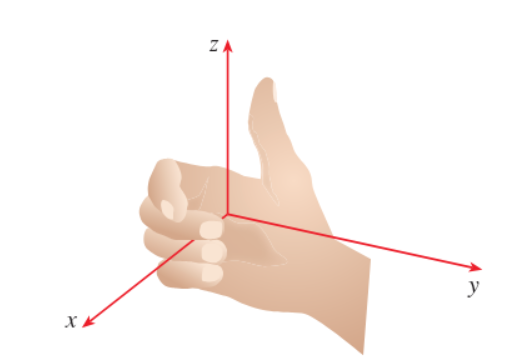
\includegraphics[width=0.5\textwidth]{images/right_hand_rule.png}
\end{center}

Projection of a point $(x, y, z)$ onto
\begin{itemize}
    \item $x-y$ plane: (x, y, 0)
    \item $x-z$ plane: (x, 0, z)
    \item $y-z$ plane: (0, y, z)
\end{itemize} 

\textbf{Distance formula in 3 dimensions:} Between two points $(x_1, y_1, z_1)$ and 
$(x_2, y_2, z_2)$, the distance is given by:
\[\sqrt{(x_2 - x_1)^2 + (y_2 - y_1)^2 +(z_2 - z_1)^2}\]

\textbf{Equation of a Sphere} with center at $(h, k, l)$ and radius $r$ is:

\[(x - h)^2 + (y - k)^2 + (z - l)^2 = r^2\]

\section{Vectors}

I will skip the basics, like vector addition definition, etc.

Components of a vector (for notation):
\[\aaa = \langle a_1, a_2, a_3 \rangle\]

Given points $A(x_1, y_1, z_1)$ and $B(x_2, y_2, z_2)$, 

\[\overrightarrow{AB} = \aaa = \langle x_2 - x_1, y_2 - y_1, z_2 - z_1 \rangle\]

\textbf{Magnitude of a vector} $\samplevec$ is 
\[|\aaa| = \sqrt{a_1^2 + a_2^2 + a_3^2}\]

\textbf{Unit vectors:} 
\[\ii = \langle 1, 0, 0 \rangle, \quad \jj = \langle 0, 1, 0 \rangle, \quad \kk = \langle 0, 0, 1 \rangle\]


\begin{tcolorbox}[colback=blue!5!white, colframe=blue!75!black, title=Algebraic Properties of Vectors in $\Rn$]
$\forall$ $\uu, \vv, \ww \in \Rn$ and scalars $c$ and $d$:
\begin{enumerate}
    \item \textbf{Commutativity of addition:} $\uu + \vv = \vv + \uu$
    \item \textbf{Associativity of addition:} $\uu + (\vv + \ww) = (\uu + \vv) + \ww$
    \item \textbf{Additive identity:} $\uu + \0 = \uu$
    \item \textbf{Additive inverse:} $\uu + (-\uu) = \0$
    \item \textbf{Distributivity of scalar multiplication over addition (vectors):} $c(\uu + \vv) = c\uu + c\vv$
    \item \textbf{Distributivity of scalar multiplication over addition (scalars):} $(c + d)\uu = c\uu + d\uu$
    \item \textbf{Associativity of scalar multiplication:} $(cd)\uu = c(d\uu)$
    \item \textbf{Scalar identity:} $1 \uu = \uu$
\end{enumerate}
\end{tcolorbox}

\section{The Dot Product}

\begin{definition}
If $\samplevec$ and $\bb = \langle b_1, b_2, b_3\rangle$ then the \textbf{dot product}
of $\aaa $ and $\bb$ is 
\[
\aaa \cdot \bb = a_1 b_1 + a_2 b_2 + a_3 b_3
\]
\end{definition}

\begin{tcolorbox}[colback=red!5!white, colframe=red!75!black, title=Properties of the Dot Product]
$\forall$ vectors $\aaa, \bb, \cc$ and scalar $c$:
\begin{enumerate}
    \item $\aaa \cdot \aaa = |\aaa|^2$
    \item $\aaa \cdot \bb = \bb \cdot \aaa$
    \item $\aaa \cdot (\bb + \cc) = \aaa \cdot \bb + \aaa \cdot \cc$
    \item $(c \aaa) \cdot \bb = c (\aaa \cdot \bb) = \aaa \cdot (c \bb)$
    \item $\0 \cdot \aaa = 0$
\end{enumerate}
\end{tcolorbox}

\begin{theorem}
    If $\theta$ is the angle between two vectors $\aaa, \bb$ then 
    \[\aaa \cdot \bb = |\aaa| |\bb| \cos \theta\]
\end{theorem}

\begin{corollary}
    Two vectors $\aaa, \bb$ are orthogonal iff $\aaa \cdot \bb = 0$
\end{corollary}

The \textbf{direction angles} of a non-zero vector $\aaa$ are the angles 
$\alpha, \beta, \gamma$ that $\aaa$ makes with the positive $x$-, $y$-, and $z$-axes, respectively.

The cosines of these angles are called \textbf{direction cosines}:

\[\cos \alpha = \frac{\aaa \cdot \ii}{|\aaa||\ii|} = \frac{a_1}{|\aaa|},
\quad \cos \beta = \frac{a_2}{|\aaa|},
\quad \cos \gamma = \frac{a_3}{|\aaa|}\]

Some nice properties of direction cosines:

\[\cos^2 \alpha + \cos^2 \beta + \cos^2 \gamma = 1\]

\[\frac{\aaa}{|\aaa|} = \langle \cos \alpha, \cos \beta, \cos \gamma \rangle\]

\textbf{Projections:}

The \textbf{projection of} $\bb$ \textbf{onto} $\aaa$ means we drop a perpendicular 
from the tip of $\bb$ onto the line spanned by $\aaa$. The resulting vector is called 
the vector projection of $\bb$ onto $\aaa$.
\\

The \textbf{scalar projection of} $\bb$ \textbf{onto} $\aaa$ is the length of this 
projection, given by
\[
\text{comp}_{\aaa} \bb = |\bb|\cos\theta = \frac{\aaa \cdot \bb}{|\aaa|},
\]
where $\theta$ is the angle between $\aaa$ and $\bb$.
\\

The \textbf{vector projection} of $\bb$ onto $\aaa$ is obtained by multiplying the 
unit vector in the direction of $\aaa$ by the scalar projection:
\[
\text{proj}_{\aaa} \bb = \left(\text{comp}_{\aaa} \bb \right)\frac{\aaa}{|\aaa|} 
= \frac{\aaa \cdot \bb}{|\aaa|^2}\aaa
\]

\section{The Cross Product}

\begin{definition}
For $\samplevec$ and $\bb = \langle b_1, b_2, b_3 \rangle$, the \textbf{cross product}
of $\aaa$ an $\bb$ is:
\[\aaa \times \bb = \langle a_2 b_3 - a_3 b_2, a_3 b_1 - a_1 b_3, a_1 b_2 - a_2 b_1 \rangle = \begin{vmatrix}
\mathbf{i} & \mathbf{j} & \mathbf{k} \\
a_1 & a_2 & a_3 \\
b_1 & b_2 & b_3
\end{vmatrix}
\]
\end{definition}

\begin{theorem}
    The vector $\aaa \times \bb$ is orthogonal to both $\aaa$ and $\bb$
\end{theorem}

\begin{theorem}
    The length of the cross product is given by: 
    \[ |\aaa \times \bb| = |\aaa| |\bb| \sin \theta\]
    where $\theta$is the angle between $\aaa$ and $\bb$.
\end{theorem}

\begin{corollary}
    Two nonzeros vectors $\aaa$ and $\bb$ are parallel iff 
    \[\aaa \times \bb = \0\]
\end{corollary}

\textbf{Area of parallelogram} determined by $\aaa$ and $\bb$ is $|\aaa \times \bb|$
\\

\textbf{Area of triangle} determined by $\aaa$ and $\bb$ is $\frac{1}{2}|\aaa \times \bb|$
\\

\textbf{IMPORTANT:} cross product is NOT commutative, and associative law for multiplication does not usually hold.

\begin{tcolorbox}[colback=red!5!white, colframe=red!75!black, title=Properties of the Cross Product]
$\forall$ vectors $\aaa, \bb, \cc$ and scalar $c$:
\begin{enumerate}
    \item $\aaa \times \bb = - \bb \times \aaa$
    \item $(c \aaa) \times \bb = c(\aaa \times \bb) = \aaa \times (c \bb)$
    \item $\aaa \times (\bb + \cc) = \aaa \times \bb + \aaa \times \cc$
    \item $(\aaa + \bb) \times \cc = \aaa \times \cc + \bb \times \cc$
    \item $\aaa \cdot (\bb \times \cc) = (\aaa \times \bb) \cdot \cc$
    \item $\aaa \times (\bb \times \cc) = (\aaa \cdot \cc) \bb - (\aaa \cdot \bb) \cc$
\end{enumerate}
\end{tcolorbox}

\textbf{Triple products:}

\[\aaa \cdot (\bb \times \cc) = \begin{vmatrix}
    a_1 & a_2 & a_3 \\
    b_1 & b_2 & b_3 \\
    c_1 & c_2 & c_3 \\
\end{vmatrix}\]


\textbf{Volume of the parallelepiped} determined by the vectors $\aaa, \bb$ and $\cc$
is:
\[V = |\aaa \cdot (\bb \times \cc)|\]

Useful: if the volume is 0, then the vectors must lie in the same plane, i.e. \textbf{coplanar}

\section{Equations of Lines and Planes}

\subsection{Equation of Lines}

\textbf{The equation of a line} that goes through point with position vector $\rr_0$, 
and is parallel to vector $\vv$ is \[
\rr = \rr_0 + t \vv
\]

If $\vv = \langle a, b, c\rangle$, $\rr_0 = \langle x_0, y_0, z_0 \rangle$ then 
\[
\langle x, y, z\rangle =  \langle x_0 + t a, y_0 + t b, z_0 + t c\rangle
\].

\textbf{Parametric form:}
\[
x = x_0 + t a \quad y = y_0 + t b \quad z = z_0 + t c
\]

\textbf{Direction numbers} of a line L are the numbers $a, b, c$ from above. 
\\

\textbf{Symmetric form:} (eliminating $t$) 
\[
\frac{x - x_0}{a} = \frac{y - y_0}{b} = \frac{z - z_0}{c}
\]

IMPORTANT: If $a, b$ or $c$ is zero, then we cannot divide by them.
For example, if $a = 0$ then the equation becomes:

\[
x = x_0, \quad \frac{y - y_0}{b} = \frac{z - z_0}{c}
\]

In general, the symmetric equations between two points $P_0(x_0, y_0, z_0), P_1(x_1, y_1, z_1)$ are 
\[
\frac{x - x_0}{x_1 - x_0} = \frac{y - y_0}{y_1 - y_0} = \frac{z - z_0}{z_1 - z_0}
\]

\textbf{The line segment} from $\rr_0$ to $\rr_1$ is given by the vector equation:
\[
\rr(t) = (1 - t)\rr_0 + t \rr_1 \quad \quad 0 \le t \le 1
\]

\subsection{Equation of Planes}

Let: 
\begin{itemize}
    \item $\mathbf{n} = \langle a, b, c \rangle$: vector orthogonal to plane
    \item $\rr_0 = \langle x_0, y_0, z_0 \rangle$: a position vector for a point in the plane 
    \item $\rr = \langle x, y, z \rangle$: a position vector for an arbitrary point in the plane.
\end{itemize}

Then the \textbf{vector equation of the plane} is: 
\[
\mathbf{n} \cdot (\rr - \rr_0) = 0 \quad \text{or} \quad \mathbf{n} \cdot \rr = \mathbf{n} \cdot \rr_0
\]

The \textbf{scalar equation} is:
\[
a(x - x_0) + b(y - y_0) + c(z - z_0) = 0
\]

The \textbf{linear equation} is:
\[
ax + by + cz - (a x_0 + b y_0 + c z_0) = 0
\] 

Two planes are parallel if their normal vectors are parallel.

If two planes are not parallel, then they intersect in a straight line and the angle between the two planes 
is defined as the acute angle between their normal vectors.

The \textbf{distance} $D$ from point $(x_1, y_1, z_1)$ to the plane 
$ax + by + cz + d = 0$ is 
\[
D = \frac{|a x_1 + b y_1 + c z_1 + d|}{\sqrt{a^2 + b^2 + c^2}}
\]

\chapter{Vector Function}

Not coming in midterm 1 $:)$

\chapter{Partial Derivatives}

\section{Functions of Several Variables}
Not coming in midterm 1 $:)$

\section{Limits and Continuity}
Not coming in midterm 1 $:)$

\section{Partial Derivatives}

If $f$ is a function of two variables, its \textbf{partial derivatives} are the functions 
$f_x, f_y$ defined by \[
f_x(x, y) = \lim_{h \to 0} \frac{f(x+h, y) - f(x, y)}{h}\]
and \[f_y(x, y) = \lim_{h \to 0} \frac{f(x, y+h) - f(x, y)}{h}\]

Also written: 
\[
f_x(x, y) = \frac{\partial f}{\partial x} = \frac{\partial z}{\partial x}
\]

\textbf{Rules for finding the partial derivatives of } $z = f(x, y)$
\begin{itemize}
    \item To find $\parx$ regard $y$ as a constant and differentiate $f(x, y)$ with respect to $x$
    \item To find $\pary$ regard $x$ as a constant and differentiate $f(x, y)$ with respect to $y$
\end{itemize}

\textbf{Interpretation of partial derivatives:}

The partial derivatives represent the instantaneous rate of change of the function's output with respect to one variable, while all other variables are held constant.
\begin{itemize}
    \item $f_x(x,y)$ is the rate at which $f$ changes with respect to $x$ when $y$ is fixed.
    \item $f_y(x,y)$ is the rate at which $f$ changes with respect to $y$ when $x$ is fixed.
\end{itemize}

\textbf{Higher Derivatives}: we can take second partial derivatives of $f$. Here is the notation:
\begin{align*}
(f_x)_x = f_{xx} &= \frac{\partial^2 f}{\partial x^2} \\
(f_x)_y = f_{xy} &= \frac{\partial^2 f}{\partial y \partial x} \\
(f_y)_x = f_{yx} &= \frac{\partial^2 f}{\partial x \partial y} \\
(f_y)_y = f_{yy} &= \frac{\partial^2 f}{\partial y^2}
\end{align*}


\begin{theorem}
\textbf{Clairaut's Theorem:} Suppose $f$ is defined on a disk $D$ that contains the 
point $(a, b)$. If $f_{xy}$ and $f_{yx}$ are both continuous on $D$, then: 
\[
f_{xy}(a, b) = f_{yx}(a, b)
\]
\end{theorem}

\section{Tangent Planes and Linear Approximations}

The equation of a \textbf{tangent plane} to the surface $z = f(x, y)$ at the point $P(x_0, y_0, z_0)$ is 
\[
z - z_0 = \parx(x_0, y_0) (x - x_0) + \pary(x_0, y_0) (y - y_0)
\]
if $f$ has continuous partial derivatives.
\\

\textbf{The Linear Approximation of} $f$ at $(a, b)$ is:
\[f(x, y) \approx f(a, b) + \parx(a, b) (x- a) + \pary(a, b) (y-b)\]

Remark: The section in the book about differentiability with epsilon has been omitted for brevity.

\begin{theorem}
If partial derivatives of $f$ exist near $(a, b)$ and are continuous at $(a, b)$ then $f$ is differentiable at $(a, b)$
\end{theorem}

\textbf{Total differential} $dz$ is defined as
\[
dz = \parx dx + \pary dy
\]

\begin{center}
    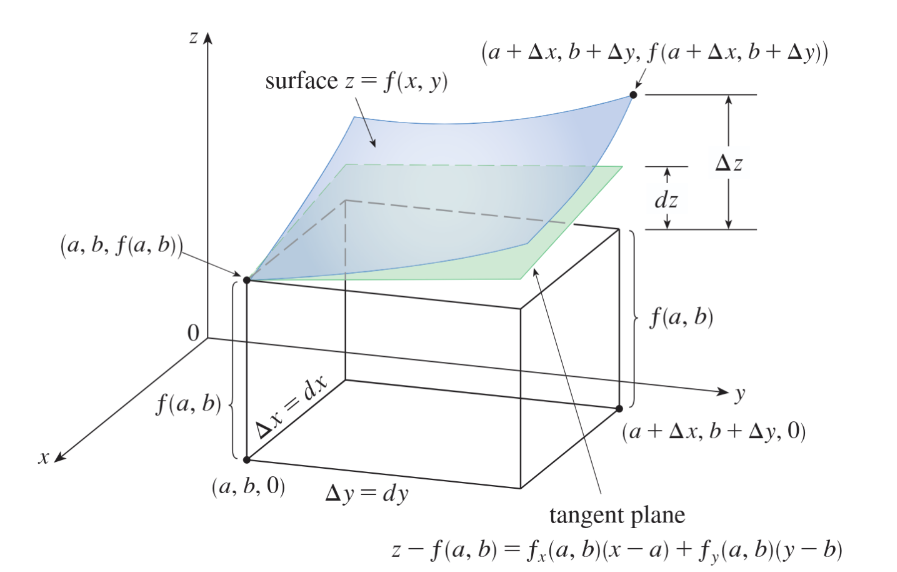
\includegraphics[width=0.5\textwidth]{images/differential.png}
\end{center}

\section{Chain Rule}

\textbf{Basic chain rule reminder:} $\frac{dy}{dt} = \frac{dy}{dx} \frac{dx}{dt}$
\\

\textbf{Chain Rule Case 1}: If $z = f(x, y)$ is a differentiable function of $x$ and $y$ which are 
both differentiable functions of $t$. Then $z$ is a differentiable function of $t$ and 
\[
\frac{dz}{dt} = \parx \frac{dx}{dt} + \pary \frac{dy}{dt}
\]

\textbf{Chain Rule Case 2}: If $z = f(x, y)$ is a differentiable function of $x$ and $y$ which are 
both differentiable functions of $s$ and $t$. Then 
\[
\frac{\partial z}{\partial s} = \parx \frac{\partial x}{\partial s} + \pary \frac{\partial y}{\partial s} \quad \quad \frac{\partial z}{\partial t} = \parx \frac{\partial x}{\partial t} + \pary \frac{\partial y}{\partial t}
\]

\begin{center}
    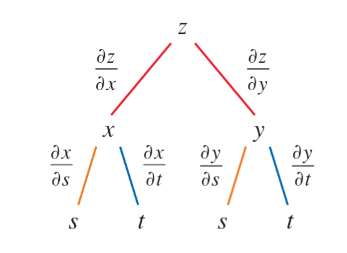
\includegraphics[width=0.5\textwidth]{images/chain.png}
\end{center}

\textbf{Chain Rule General Case}: If 
\begin{itemize}
    \item $u$ is a differentiable function of $n$ variables $x_1, \dots, x_n$
    \item Each $x_i$ is a differentiable function of $m$ variables $t_1, \dots, t_m$
\end{itemize}
Then $u$ is a function of $t_1, \dots, t_m$ and 
\[
\frac{\partial u}{\partial t_i} = \frac{\partial u}{\partial x_1} \frac{\partial x_1}{\partial t_i} + \dots + \frac{\partial u}{\partial x_n} \frac{\partial x_n}{\partial t_i}
\]
for all $i = 1, \dots, m$


\end{document}